\section{《概率论与数理统计》期中考试}

\subsection{选择题(每小题3分,共15分)}

\begin{question}{题目1}
    $A, B, C$ 是相互独立的三个事件且 $P(A) = P(B) = P(C) = 0.3$,则 $P(A \cup B \cup C)$ 的值为 (\quad \quad)
    \begin{multicols}{4}
        \begin{itemize}
            \item [(A)] 0.9
            \item [(B)] 0.3
            \item [(C)] 0.027
            \item [(D)] 0.657
        \end{itemize}
    \end{multicols}
\end{question}
\begin{solution}
    选(D).  根据三个事件的概率加法公式和事件的独立性,有
    $$
        \begin{aligned}
            P(A \cup B \cup C)
             & = P(A) + P(B) + P(C) - P(AB) - P(AC) - P(BC) + P(ABC)                \\
             & = P(A) + P(B) + P(C) - P(A)P(B) - P(A)P(C) - P(B)P(C) + P(A)P(B)P(C) \\
             & = 0.3 + 0.3 + 0.3 - 0.09 - 0.09 - 0.09 + 0.027                       \\
             & = 0.657.                                                             \\
        \end{aligned}
    $$
\end{solution}


\begin{question}{题目2}
    设随机变量 $X \sim N(0,1)$ , $X$ 的分布函数为 $\Phi(x)$,则 $P\{|X|>2\}$ 的值为 (\quad \quad)
    \begin{multicols}{4}
        \begin{itemize}
            \item [(A)] $2[1 - \Phi(2)]$
            \item [(B)] $2\Phi(2) - 1$
            \item [(C)] $2 - \Phi(2)$
            \item [(D)] $1 - 2\Phi(2)$
        \end{itemize}
    \end{multicols}
\end{question}
\begin{solution}
    选(A).  根据正态分布函数的定义:
    $$
        \Phi(x) = P\{X \leqslant x\},
    $$
    和正态分布的对称性
    $$
        \Phi(-x) = 1 - \Phi(x),
    $$
    得到
    $$
        \begin{aligned}
            P\{|X|>2\}
             & = P\{X<-2\} + P\{X>2\}                 \\
             & = P\{X<-2\} + (1 - P\{X \leqslant 2\}) \\
             & = \Phi(-2) + [1 - \Phi(2)]             \\
             & = [1 - \Phi(2)] + [1 - \Phi(2)]        \\
             & = 2[1 - \Phi(2)].                      \\
        \end{aligned}
    $$
\end{solution}


\begin{question}{题目3}
    设随机变量 $X \sim \pi(2)$,则 $P\{X \leqslant 1\}$ 的值为 (\quad \quad)
    \begin{multicols}{4}
        \begin{itemize}
            \item [(A)] $\mathrm{e}^{-2}$
            \item [(B)] $2\mathrm{e}^{-2}$
            \item [(C)] $3\mathrm{e}^{-2}$
            \item [(D)] $4\mathrm{e}^{-2}$
        \end{itemize}
    \end{multicols}
\end{question}
\begin{solution}
    选(C). 根据泊松分布的定义
    $$
        P\{X=k\} = \frac{\lambda^k\mathrm{e}^{-\lambda}}{k!}.
    $$
    当 $\lambda = 2$ 时,有
    $$
        P\{X \leqslant 1\}
        = P\{X = 0\} + P\{X = 1\}
        = \frac{2^0 \mathrm{e}^{-2} }{0!} + \frac{2^1 \mathrm{e}^{-2} }{1!}
        = 3\mathrm{e}^{-2}.
    $$
\end{solution}


\begin{question}{题目4}
    一盒中有3个红球,1个白球,不放回取2个球,$X$ 表示取到的红球数,$F(x)$ 是 $X$ 的分布函数,则 $F(1.5)$ 的值为 (\quad \quad)
    \begin{multicols}{4}
        \begin{itemize}
            \item [(A)] 0
            \item [(B)] 0.25
            \item [(C)] 0.5
            \item [(D)] 0.75
        \end{itemize}
    \end{multicols}
\end{question}
\begin{solution}
    选(C).  根据分布函数的定义:
    $$
        F(x) = P\{X \leqslant x\}.
    $$
    有
    $$
        F(1.5) = P\{X \leqslant 1.5\}
        = P\{X=0\} + P\{X=1\}
        = 0 + \frac{C_3^1C_1^1}{C_4^2}
        = \frac{1}{2}.
    $$
\end{solution}

\begin{question}{题目5}
    已知 $(X,Y)$ 的联合分布律为 $P\{X=1, Y=1\} = 0.1$,$P\{X=1, Y=2\} = 0.3$,$P\{X=2, Y=1\}=0.4$,$P\{X=2, Y=2\}=0.2$,$F(x,y)$ 是 $(X,Y)$ 的分布函数,$F_X(x)$ 是 $X$ 的边际分布函数,则以下结果正确的是 (\quad \quad)
    \begin{multicols}{4}
        \begin{itemize}
            \item [(A)] $F(1.5, 2) = 0.1$
            \item [(B)] $F_X(2.5) = 1$
            \item [(C)] $F_X(1.5) = 0$
            \item [(D)] $F(2,2) = 0.2$
        \end{itemize}
    \end{multicols}
\end{question}
\begin{solution}
    选(B).  二维随机变量的 $(X,Y)$ 联合分布函数定义为
    $$
        F(x,y) = P\{X \leqslant x, Y \leqslant y\}.
    $$
    二维随机变量 $(X,Y)$ 关于 $X$ 和关于 $Y$ 的边缘分布函数定义为
    $$
        F_X(x) = P\{X \leqslant x\}
        = P\{X \leqslant x, Y < +\infty\}
        = F(x, +\infty).
    $$
    $$
        F_Y(y) = P\{Y \leqslant y\}
        = P\{X \leqslant +\infty, Y < y\}
        = F(+\infty, y).
    $$
    对于选项(A)
    $$
        \begin{aligned}
            F(1.5, 2)
             & = P\{X \leqslant 1.5, Y \leqslant 2\} \\
             & = P\{X=1, Y=1\} + P\{X=1, Y=2\}       \\
             & = 0.1 + 0.3                           \\
             & = 0.4.                                \\
        \end{aligned}
    $$
    对于选项(B)
    $$
        \begin{aligned}
            F_X(2.5)
             & = P\{X \leqslant 2.5, Y \leqslant +\infty\}                     \\
             & = P\{X=1, Y=1\} + P\{X=1, Y=2\} + P\{X=2, Y=1\} + P\{X=2, Y=2\} \\
             & = 0.1+0.3+0.4+0.2                                               \\
             & = 1.                                                            \\
        \end{aligned}
    $$
    对于选项(C)
    $$
        F_X(1.5) = P\{X=1, Y=1\} + P\{X=1, Y=2\} = 0.1 + 0.3 = 0.4.
    $$
    对于选项(D)
    $$
        \begin{aligned}
            F(2,2)
             & = P\{X \leqslant 2, Y \leqslant 2\}                             \\
             & = P\{X=1, Y=1\} + P\{X=1, Y=2\} + P\{X=2, Y=1\} + P\{X=2, Y=2\} \\
             & = 0.1+0.3+0.4+0.2                                               \\
             & = 1.                                                            \\
        \end{aligned}
    $$
\end{solution}


\subsection{填空题(每小题3分,共15分)}

\begin{question}{题目6}
    已知 $P(A \cup B) = 0.7$,$P(A) = 0.4$,当 $A$ 与 $B$ 不相容时,$P(B) = $ \underline{\hspace{2cm}}.
\end{question}
\begin{solution}
    根据概率的加法公式和事件 $A,B$ 互不相容,有
    $$
        \begin{cases}
            P(A \cup B)  = P(A) + P(B) - P(AB), \\
            P(AB) = P(\varnothing) = 0.         \\
        \end{cases}
        \implies
        P(B) = 0.3.
    $$
\end{solution}

\begin{question}{题目7}
    已知 $(X,Y)$ 的联合分布律为
    $$
        %\renewcommand\arraystretch{1.8}
        \setlength{\arraycolsep}{10mm}
        \begin{array}{c|ccccc}
            X \setminus Y & -1   & 0    & 1    \\
            \hline
            -1            & 1/18 & 2/18 & 0    \\
            0             & 3/18 & 4/18 & 5/18 \\
            2             & 0    & 2/18 & 1/18 \\
        \end{array}
    $$
    则 $P\{X \leqslant 0 , |Y|<1\} = $ \underline{\hspace{2cm}}.
\end{question}
\begin{solution}
    $$
        \begin{aligned}
            P\{X \leqslant 0 , |Y|<1\}
             & = P\{X \leqslant 0 , -1<Y<1\}    \\
             & = P\{X=-1, Y=0\} + P\{X=0, Y=0\} \\
             & = \frac{2}{18} + \frac{4}{18}    \\
             & = \frac{1}{3}.                   \\
        \end{aligned}
    $$
\end{solution}

\begin{question}{题目8}
    设随机变量 $X$ 服从参数 $\theta = 2$ 的指数分布,则 $P\{X \geqslant 2\} = $ \underline{\hspace{2cm}}.
\end{question}
\begin{solution}
    随机变量 $X$ 服从参数 $\theta = 2$ 的指数分布
    $$
        f(x) = \begin{dcases}
            \frac{1}{2}\mathrm{e}^{-\frac{x}{2}}, & x>0,       \\
            0,                                    & \text{其他}. \\
        \end{dcases}
    $$
    在对应区间积分,得到
    $$
        P\{X\geqslant2\}
        = \int_{2}^{+\infty} \frac{1}{2} \mathrm{e}^{-\frac{x}{2}} \,\mathrm{d}x
        = -\int_{2}^{+\infty} \mathrm{e}^{-\frac{x}{2}} \mathrm{d}\left(-\frac{x}{2}\right)
        = -\left(\mathrm{e}^{-\frac{x}{2}}\Big|_{2}^{+\infty}\right)
        = \mathrm{e}^{-1}.
    $$
\end{solution}


\begin{question}{题目9}
    设随机变量 $X \sim  N(0,4)$,其概率密度函数为 $f_1(x)$,随机变量 $Y \sim U(-1,4)$,其概率密度函数为 $f_2(y)$. 若 $f(x) = \begin{cases} af_1(x), & x \leqslant 0, \\ bf_2(x), & x>0.\end{cases}$ 是概率密度函数,其中 $a>0, b>0$,则 $a,b$ 应满足 \underline{\hspace{2cm}}.
\end{question}
\begin{solution}
    根据概率密度的性质
    $$
        \int_{-\infty}^{+\infty} f(x) \ \mathrm{d}x = 1.
    $$
    有
    $$
        \begin{aligned}
            \int_{-\infty}^{+\infty} f(x)\,\mathrm{d}x
              & =\int_{-\infty}^{0} af_1(x)\,\mathrm{d}x+\int_{0}^{+\infty} bf_2(x) \,\mathrm{d}x                                          \\
            1 & =a\int_{-\infty}^{0}\frac{1}{\sqrt{2\pi}}\mathrm{e}^{-\frac{x^2}{8}}\,\mathrm{d}x+b\int_{0}^{4}\frac{1}{4-(-1)}\mathrm{d}x \\
            1 & =\frac{a}{2} + \frac{4b}{5}.
        \end{aligned}
    $$
    综上, $a,b$ 满足 $5a+8b=10.$
\end{solution}


\begin{question}{题目10}
    随机变量 $X$ 在区间 $(1,3)$ 上服从均匀分布,对 $X$ 独立重复观察 3 次,则至少有 2 次观测值大于 1.5 的概率为 \underline{\hspace{2cm}}.
\end{question}
\begin{solution}
    随机变量 $X$ 的概率密度为
    $$
        f(x) = \begin{dcases}
            \frac{1}{2}, & 1<x<3,     \\
            0,           & \text{其他}.
        \end{dcases}
    $$
    观测值大于 1.5 的概率为
    $$
        P\{X \geqslant 1.5\} = \int_{1.5}^{3} \frac{1}{2} \,\mathrm{d}x = \frac{3}{4}.
    $$
    对 $X$ 独立重复观察 3 次,至少有 2 次观测值大于 1.5 的概率为
    $$
        P = C_3^2\left(\frac{3}{4}\right)^2\left(\frac{1}{4}\right)^1 + C_3^3\left(\frac{3}{4}\right)^3\left(\frac{1}{4}\right)^0
        = \frac{27}{32}.
    $$
\end{solution}


\subsection{计算题(共70分)}

\begin{question}{题目11(10分)}
    福建师范大学实验幼儿园举行家长开放日活动,小浩家参加活动的家长是父亲或者母亲. 父亲参加的概率是 0.9,若父亲参加,则母亲参加的概率为 0.1;若父亲没有参加,则母亲参加的概率为 0.5. 求:

    \begin{itemize}
        \item [(1)] 母亲参加的概率.
        \item [(2)] 在已知母亲参加的条件下,父亲参加的概率.
    \end{itemize}
\end{question}
\begin{solution}
    设事件 $A$ 为父亲参加开放日,事件 $B$ 为母亲参加开放日.
    $$
        \begin{cases}
            P(A) = 0.9,              & P(\overline{A}) = 0.1,              \\
            P(B|A) = 0.9,            & P(\overline{B}|A) = 0.1,            \\
            P(B|\overline{A}) = 0.5, & P(\overline{B}|\overline{A}) = 0.5. \\
        \end{cases}
    $$
    (1) 根据全概率公式,母亲参加的概率为
    $$
        P(B) = P(B|A)P(A) + P(B|\overline{A})P(\overline{A})
        = 0.1 \times 0.9 + 0.5 \times 0.1
        = 0.14.
    $$
    (2) 根据贝叶斯公式,在已知母亲参加的条件下,父亲参加的概率为
    $$
        \begin{aligned}
            P(A|B)
             & = \frac{P(B|A_i)P(A_i)}{\sum\limits_{j=1}^2 P(B|A_j)P(A_j)}        \\
             & = \frac{P(B|A)P(A)}{P(B|A)P(A) + P(B|\overline{A})P(\overline{A})} \\
             & = \frac{0.1 \times 0.9}{0.1 \times 0.9 + 0.5 \times 0.1}           \\
             & = \frac{9}{14}.                                                    \\
        \end{aligned}
    $$
\end{solution}

\begin{question}{题目12(10分)}
    在一次打靶训练中,某运动员给自己定的目标是要一直打到命中 10 环为止. 已知他每次命中 10 环的概率为 $p$,$0<p<1$. 设各次是否命中相互独立,求:
    \begin{itemize}
        \item [(1)] 他打靶次数的分布律.
        \item [(2)] 如果他打了 $n$ 次还没有命中,还需要进行 $m$ 次的概率.
        \item [(3)] 如果他打了 5 分钟还没有命中,还需要进行 $m$ 次的概率.
    \end{itemize}
\end{question}
\begin{solution}
    (1) 用随机变量 $X$ 表示打靶的次数,其分布律为
    $$
        P\{X=k\} = (1-p)^{k-1}p.
    $$
    (2) 用随机变量 $X$ 表示已经射击的次数,$Y$ 表示继续射击的次数,结合条件概率公式,有
    $$
        \begin{aligned}
            P\{Y=m|X=n\}
             & = \frac{P\{Y=m, X=n\}}{P\{X=n\}} \\
             & = \frac{(1-p)^{n+m-1}p}{(1-p)^n} \\
             & = (1-p)^{m-1}p.                  \\
        \end{aligned}
    $$
    (3) 根据第(2)小题的结果,继续射击的次数与之前的射击结果没有关系
    $$
        P = (1-p)^{m-1}p.
    $$
\end{solution}

\begin{question}{题目13(12分)}
    设 $A,B$ 为随机事件,且 $P(A) = 0.3, P(B) = 0.12, P(AB) = 0.06$,令
    $$
        X = \begin{cases}
            1, & A\text{发生},  \\
            0, & A\text{不发生},
        \end{cases}
        Y = \begin{cases}
            1, & B\text{发生},  \\
            0, & B\text{不发生}.
        \end{cases}
    $$
    求 $(X,Y)$ 的联合概率密度及边缘分布律.
\end{question}
\begin{solution}
    根据事件运算的分配律
    $$
        P(A\overline{B}) = P(A(S-B)) = P(A) - P(AB) = 0.24.
    $$
    $$
        P(\overline{A}B) = P((S-A)B) = P(B) - P(AB) = 0.06.
    $$
    根据事件运算的徳摩根律
    $$
        P(\overline{AB}) = P(\overline{A \cup B})
        = 1 - [P(A) + P(B) - P(AB)]
        = 0.64.
    $$
    得到 $(X,Y)$ 的联合概率密度及边缘分布律
    $$
        %\renewcommand\arraystretch{1.5}
        %\setlength{\arraycolsep}{12mm}
        \begin{array}{c|cc|c}
            X \setminus Y & 0    & 1    & P\{X=i\} \\
            \hline
            0             & 0.64 & 0.24 & 0.88     \\
            1             & 0.06 & 0.06 & 0.12     \\
            \hline
            P\{Y=j\}      & 0.70 & 0.30 & 1        \\
        \end{array}
    $$
\end{solution}

\begin{question}{题目14(12分)}
    某化合物的酒精含量百分比 $X$ 是随机变量,其概率密度函数为:
    $$
        f(x) = \begin{cases}
            c(1-x), & 0.3<x<0.7, \\
            0,      & \text{其他.}
        \end{cases}
    $$
    此化合物的成本为每升 10 元,售价为每升 40 元或 60 元. 若 $0.4<X<0.6$ ,则售价以 0.9 的概率为 60 元,否则以概率 0.2 为 60 元. 以 $Y$ 表示每升的利润,求:
    \begin{itemize}
        \item [(1)] 常数 $c$.
        \item [(2)] $X$ 的分布函数 $F(x)$.
        \item [(3)] $Y$ 的分布律和分布函数.
    \end{itemize}
\end{question}
\begin{solution}
    (1) 根据概率密度的性质
    $$
        \int_{-\infty}^{+\infty} f(x) \,\mathrm{d}x
        = \int_{0.3}^{0.7} c(1-x) \,\mathrm{d}x
        = \left.c\left(x-\frac{1}{2}x^2\right)\right|_{0.3}^{0.7}
        = 1,
    $$
    解得
    $$
        c = 5.
    $$
    (2) 分布函数 $F(x)$ 定义为
    $$
        F(x) = \int_{-\infty}^{x} f(x) \,\mathrm{d}x.
    $$
    \paragraph{情形一} 当 $x \leqslant 0.3$ 时
    $$
        F(x) = \int_{-\infty}^{x} 0 \,\mathrm{d}x = 0.
    $$
    \paragraph{情形二} 当 $0.3<x<0.7$ 时
    $$
        F(x) = \int_{-\infty}^{0.3} 0\,\mathrm{d}x + \int_{0.3}^x 5(1-x)\,\mathrm{d}x
        = \left.\left(-\frac{5}{2}x^2 + 5x\right)\right|_{0.3}^{x}
        = -\frac{5}{2}x^2 + 5x - \frac{51}{40}.
    $$
    \paragraph{情形三} 当 $x \geqslant 0.7$ 时
    $$
        F(x) = \int_{-\infty}^{0.3}0\,\mathrm{d}x + \int_{0.3}^{0.7}5(1-x)\,\mathrm{d}x + \int_{0.7}^{x} 0\,\mathrm{d}x = 1.
    $$
    综上所述,分布函数 $F(x)$ 为
    $$
        F(x) = \int_{-\infty}^x f(x) \,\mathrm{d}x
        = \begin{dcases}
            0,                                    & x \leqslant \frac{3}{10},    \\
            -\frac{5}{2}x^2 + 5x - \frac{51}{40}, & \frac{3}{10}<x<\frac{7}{10}, \\
            1,                                    & x \geqslant \frac{7}{10}.
        \end{dcases}
    $$
    (3) 根据全概率公式,有
    $$
        \begin{aligned}
            P\{Y=50 , 0.4<X<0.6\}
             & = P\{Y=30 | 0.4<X<0.6\}P\{0.4<X<0.6\} \\
             & = 0.9 [F(0.6)-F(0.4)]                 \\
             & = 0.9 \times 0.5                      \\
             & = 0.45.                               \\
        \end{aligned}
    $$
    $$
        \begin{aligned}
            P\{Y=30, 0.4<X<0.6\}
             & = P\{Y=30 | 0.4<X<0.6\}P\{0.4<X<0.6\} \\
             & = 0.1 [F(0.6)-F(0.4)]                 \\
             & = 0.1 \times 0.5                      \\
             & = 0.05.                               \\
        \end{aligned}
    $$
    $$
        \begin{aligned}
            P\{Y=50 , X \notin (0.4,0.6)\}
             & = P\{Y=50 |  X \notin (0.4,0.6)\}P\{X \notin (0.4,0.6)\} \\
             & = 0.2 [F(0.4)-F(0.3) + F(0.7)-F(0.6)]                    \\
             & = 0.2 \times 0.5                                         \\
             & = 0.1.                                                   \\
        \end{aligned}
    $$
    $$
        \begin{aligned}
            P\{Y=30 , X \notin (0.4,0.6)\}
             & = P\{Y=30 |  X \notin (0.4,0.6)\}P\{X \notin (0.4,0.6)\} \\
             & = 0.8 [F(0.4)-F(0.3) + F(0.7)-F(0.6)]                    \\
             & = 0.8 \times 0.5                                         \\
             & = 0.4.
        \end{aligned}
    $$
    $$
        P\{Y=50\} = P\{Y=50 , 0.4<X<0.6\} + P\{Y=50 , X \notin (0.4,0.6)\} = 0.55.
    $$
    $$
        P\{Y=30\} = P\{Y=30, 0.4<X<0.6\} + P\{Y=30 , X \notin (0.4,0.6)\} = 0.45.
    $$
    综上,$Y$ 的分布律为
    $$
        \begin{array}{c|ccc}
            Y   & 30   & 50   \\
            \hline
            p_k & 0.45 & 0.55
        \end{array}
    $$
    分布函数 $F(y)$ 为
    $$
        F(y) = \begin{dcases}
            0,            & y < 30,              \\
            \frac{9}{20}, & 30 \leqslant y < 50, \\
            1,            & y \geqslant 50.
        \end{dcases}
    $$
\end{solution}

\begin{question}{题目15(12分)}
    设 $X$ 的概率密度
    $$
        f(x) = \begin{dcases}
            \frac{1}{4}, & -2 < x< 0,         \\
            \frac{1}{6}, & 0 \leqslant x < 3, \\
            0,           & \text{其他}.
        \end{dcases}
    $$
    令 $Y=X^4$,求:
    \begin{itemize}
        \item [(1)] $Y$ 的概率密度 $f_Y(y)$.
        \item [(2)] $P\left\{X \leqslant -\dfrac{1}{2}, Y \leqslant 1\right\}$.
    \end{itemize}
\end{question}
\begin{solution}
    (1) 根据分布函数的定义
    $$
        \begin{aligned}
            F_Y(y)
            = P\{Y \leqslant y\}
            = P\left\{X^4 \leqslant y\right\}
            = P\left\{-y^\frac{1}{4} \leqslant X \leqslant y^\frac{1}{4}\right\}
            = F_X\left(y^\frac{1}{4}\right)-F_X\left(-y^\frac{1}{4}\right),
        \end{aligned}
    $$
    将 $F_Y(y)$ 对 $y$ 求导得到 $f_Y(y)$
    $$
        \begin{aligned}
            f_Y(y) = F_Y'(y)
             & = F_X'\left(y^\frac{1}{4}\right) - F_X'\left(-y^\frac{1}{4}\right)                                                                                \\
             & = f_X\left(y^\frac{1}{4}\right)\left(\frac{1}{4}y^{-\frac{3}{4}}\right) - f_X\left(-y^\frac{1}{4}\right)\left(-\frac{1}{4}y^{-\frac{3}{4}}\right) \\
             & = \frac{1}{4}y^{-\frac{3}{4}}\left[f_X\left(y^\frac{1}{4}\right) + f_X\left(-y^\frac{1}{4}\right)\right],                                         \\
        \end{aligned}
    $$
    综上,$Y$ 的概率密度函数为
    $$
        f_Y(y) = \begin{dcases}
            \frac{5}{48}y^{-\frac{3}{4}}, & 0 \leqslant y < 16,  \\
            \frac{1}{24}y^{-\frac{3}{4}}, & 16 \leqslant y < 81, \\
            0,                            & \text{其他}.           \\
        \end{dcases}
    $$
    (2)
    $$
        \begin{aligned}
            P\left\{X \leqslant -\frac{1}{2}, Y \leqslant 1\right\}
             & = P\left\{X \leqslant -\frac{1}{2}, X^4 \leqslant 1\right\}            \\
             & = P\left\{X \leqslant -\frac{1}{2}, -1 \leqslant X \leqslant 1\right\} \\
             & = P\left\{-1 \leqslant X \leqslant -\frac{1}{2}\right\}                \\
             & = \int_{-1}^{-\frac{1}{2}} \frac{1}{4} \,\mathrm{d}x                   \\
             & = \frac{1}{8}.                                                         \\
        \end{aligned}
    $$
\end{solution}


\begin{question}{题目16(14分)}
    设 $(X,Y)$ 的概率密度为
    $$
        f(x,y) = \begin{cases}
            kx^2y, & 0 \leqslant x \leqslant 1,0 \leqslant y \leqslant 1, \\
            0,     & \text{其他}.
        \end{cases}
    $$
    求:
    \begin{itemize}
        \item [(1)] 常数 $k$.
        \item [(2)] $f_X(x), f_Y(y)$.
        \item [(3)] $P\{X+Y>1\}$.
    \end{itemize}
\end{question}
\begin{solution}
    (1) 根据概率密度的性质
    $$
        \int_{-\infty}^{+\infty}\int_{-\infty}^{+\infty} f(x,y) \,\mathrm{d}x\mathrm{d}y = 1.
    $$
    结合如图所示的积分区域
    \begin{center}
        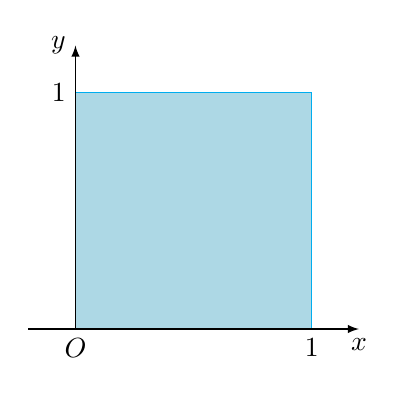
\begin{tikzpicture}[scale = 3]
            %画填充色快
            \filldraw[LightBlue] (0, 0) -- (0, 1) -- (1, 1) -- (1, 0) -- cycle;
            \draw[cyan] (0, 1) -- (1, 1) -- (1, 0);
            %标注坐标轴
            \draw[-latex] (-0.2, 0) -- (1.2, 0) node[below] {$x$};
            \draw[-latex] (0, 0) -- (0, 1.2) node[left] {$y$};
            \node[below] at (0,0) {$O$};
            %标注点
            \node[left] at (0, 1) {$1$};
            \node[below] at (1, 0)  {$1$};
        \end{tikzpicture}
    \end{center}
    得到
    $$
        \int_{0}^{1}\int_{0}^{1} kx^2y \,\mathrm{d}x\mathrm{d}y
        = \int_{0}^{1} kx^2 \mathrm{d}x \int_{0}^{1} y \,\mathrm{d}y
        = \int_{0}^{1} kx^2 \left(\left.\frac{y^2}{2}\right|_{0}^{1}\right) \mathrm{d}x
        = \left.\frac{k}{6}x^3\right|_{0}^{1}
        = 1,
    $$
    解得
    $$
        k=6.
    $$
    (2) 根据边缘概率密度的定义
    $$
        f_X(x) = \int_{-\infty}^{+\infty} f(x,y) \,\mathrm{d}y
        = \begin{dcases}
            \int_{0}^{1} 6x^2y \,\mathrm{d}y, & 0 \leqslant x \leqslant 1, \\
            0,                                & \text{其他}.
        \end{dcases}
        = \begin{cases}
            3x^2, & 0 \leqslant x \leqslant 1, \\
            0,    & \text{其他}.
        \end{cases}
    $$
    $$
        f_Y(y) = \int_{-\infty}^{+\infty} f(x,y) \,\mathrm{d}y
        = \begin{dcases}
            \int_{0}^{1} 6x^2y \,\mathrm{d}x, & 0 \leqslant y \leqslant 1, \\
            0,                                & \text{其他}.
        \end{dcases}
        = \begin{cases}
            2y, & 0 \leqslant y \leqslant 1, \\
            0,  & \text{其他}.
        \end{cases}
    $$
    (3) 新的积分区域如图所示
    \begin{center}
        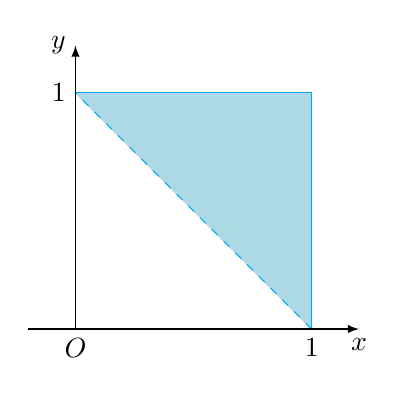
\begin{tikzpicture}[scale = 3]
            %画填充色快
            \filldraw[LightBlue] (0, 1) -- (1, 1) -- (1, 0) -- cycle;
            \draw[cyan, dashed] (1, 0) -- (0, 1);
            \draw[cyan] (0, 1) -- (1, 1) -- (1, 0);
            %标注坐标轴
            \draw[-latex] (-0.2, 0) -- (1.2, 0) node[below] {$x$};
            \draw[-latex] (0, 0) -- (0, 1.2) node[left] {$y$};
            \node[below] at (0,0) {$O$};
            %标注点
            \node[left] at (0, 1) {$1$};
            \node[below] at (1, 0)  {$1$};
        \end{tikzpicture}
    \end{center}
    根据概率密度的性质,得到
    $$
        P\{X+Y>1\}
        = \int_{0}^{1}\mathrm{d}x \int_{1-x}^1 6x^2y \,\mathrm{d}y
        = \int_{0}^{1} 3x^2\left[1-(1-x)^2\right] \,\mathrm{d}x
        = \frac{9}{10}.
    $$
\end{solution}